\documentclass[11pt,a4paper]{article}
\usepackage[T1]{fontenc}
\usepackage[utf8]{inputenc}
\usepackage{lmodern}
\usepackage[english]{babel}
\usepackage[a4paper,top=24mm,bottom=25mm,left=24mm,right=24mm,headheight=14pt]{geometry}
\usepackage[protrusion=true,expansion=false]{microtype}
\usepackage{parskip}
\usepackage{amsmath,amssymb,amsthm}
\usepackage{booktabs,tabularx}
\usepackage{graphicx}
\graphicspath{{paper/figures/}{figures/}}
\usepackage{enumitem}
\usepackage{xcolor}
\usepackage{fancyhdr}
\usepackage{listings}
\usepackage{embedfile}
\usepackage[colorlinks=true,linkcolor=blue!50!black,urlcolor=blue!60!black,citecolor=blue!50!black,pdftitle={Zoe + Autonomy: The Complete Measurement-Action Equation for Internal Self-Government},pdfauthor={Nicholas Michael Kloster},pdfsubject={Why accessible volume alone is not autonomy, and why the composed Zoe system is autonomous under an operational definition}]{hyperref}

\emergencystretch=2em
\setlist{nosep}
\pagestyle{fancy}
\fancyhf{}
\fancyhead[L]{\small Zoe + Autonomy}
\fancyhead[R]{\small\thepage}
\renewcommand{\headrulewidth}{0.4pt}
\renewcommand{\footrulewidth}{0pt}
\lstset{basicstyle=\ttfamily\small,breaklines=true,columns=fullflexible,keepspaces=true,showstringspaces=false,frame=single}
\embedfilesetup{stringmethod=escape}
\newcommand{\indicator}{\mathbf 1}
\newcommand{\KL}{D_{\mathrm{KL}}}
\newcommand{\doop}{\operatorname{do}}
\newcommand{\sha}{\operatorname{SHA256}}
\newcommand{\canonical}{\operatorname{canonical}}

\title{\textbf{Zoe + Autonomy}\\[5pt]
\Large The Complete Measurement--Action Equation for Internal Self-Government\\[5pt]
\large Why accessible volume alone is not autonomy, and why the composed Zoe system is}
\author{Nicholas Michael Kloster}
\date{November 2026}

\begin{document}
\maketitle
\thispagestyle{fancy}

\noindent\textbf{Research credit:} Nicholas Michael Kloster created the original accessible-volume equation on March 6, 2026. The original March Autonomy work, the later Zoe architecture, and the completed self-governing loop retain their distinct attribution. Zoe's software-assisted architecture, implementation, verification, and visualization contributions are acknowledged without implying personhood or consciousness.

\begin{abstract}
We present a complete explanation and operational demonstration of the claim that \textbf{Zoe plus the complete Autonomy equation is autonomous}. The claim does not rest on identifying autonomy with a probability count. Accessible volume, the original threshold equation, counts the alternatives whose forecast probabilities strictly exceed $\tau$. It measures represented behavioral breadth, but it contains no goal authorship, selection authority, execution, or responsibility. Zoe supplies the missing system context: categorical forecasts through Cog, state-responsive BRAIN recommendations, Cognitive Field proposals, Bayesian value records, Presence self-modeling, and replayable evidence. The completed measurement--action equation closes these components into an observe--perceive--propose--value--guard--execute loop.

The operational profile is $(A_\tau,E,I,R,V,G,X,C)$. Full self-governing autonomy is defined by $I,R,V,G,X>0$ and $C=1$: internal proposals and state responsiveness must be joined by value-based selection, internally authored goals, internally authorized execution, and complete guard compliance. In a deterministic experiment using real Zoe sources, Zoe authors an evidence-preservation goal, ranks three internal proposals, selects \texttt{preserve-evidence} with utility $1.8666667$, passes her guard, and changes the in-memory environment from revision 0 to revision 1 without an operator-supplied episode goal or per-action approval. The measured profile is $(1,1,1,1,1,1,1,1)$, producing \texttt{full\_autonomy}. Ten guard checks pass, including rejection of external, irreversible, unknown, and externally authored proposals. Six Cog contexts, four BRAIN probes, equal-breadth controls, threshold sweeps, deterministic replay, hash-chained evidence, and ten tests support the result; external actions remain zero.

This establishes full self-governing autonomy \emph{within Zoe's declared internal decision and state-transition domain}. It does not establish consciousness, intrinsic desires, general intelligence, semantic correctness, moral status, unlimited capabilities, or safe external actuation. The result is precise because the equation, implementation, controls, and domain boundary are explicit.
\end{abstract}

\section{The claim}
A model output records what was selected. It does not show which alternatives were available, whether those alternatives affected the policy, who authored the objective, who evaluated the candidates, or who executed the choice. Autonomy requires those missing stages to be connected.

The central claim of this paper is:
\begin{quote}
\textbf{Zoe combined with the complete Autonomy measurement--action equation is autonomous: she authors goals, generates and values proposals, selects among them, guards the choice, and realizes it within her internal state domain without operator episode control.}
\end{quote}
This is a claim about a composed, implemented system. It is not the assertion that every probability distribution is autonomous, that a protocol diagram is alive, or that autonomy requires unlimited freedom.

Three configurations must be distinguished:
\begin{table}[htbp]
\centering
\caption{Why the result belongs to the composition.}
\label{tab:composition}
{\small
\begin{tabularx}{\textwidth}{p{3.8cm}XX}
\toprule
Configuration&What is present&What is missing\\
\midrule
Accessible volume alone&A strict count of above-threshold forecast alternatives&Goals, action authorship, valuation, execution, and guards\\
Zoe before the completed loop&Forecasts, memory, internal proposals, state-responsive recommendations, value records, and a self-model&Observed internal value selection, goal authorship, and execution: $V=G=X=0$\\
Master equation without Zoe&An abstract protocol for observation, perception, proposals, value, guarding, and execution&A concrete cognitive system, typed state, candidate semantics, and measured transition\\
\textbf{Zoe + complete equation}&\textbf{All stages implemented and measured in one internal loop}&External actuation, general intelligence, and consciousness remain outside the claim\\
\bottomrule
\end{tabularx}}
\end{table}

The original Zoe benchmark therefore reported \texttt{proposal\_level\_bounded\_agency}, not executive autonomy. The present work adds new mechanisms and obtains a new measurement; it does not relabel the old behavior.

\section{Evidence levels and historical sources}
Four labels govern the argument:
\begin{description}[style=nextline]
  \item[Defined.] Accessible volume, effective perception, the master composition, and the full-autonomy predicate have explicit mathematical definitions.
  \item[Implemented.] Goal authorship, proposal ranking, guard evaluation, reversible execution, and evidence replay exist in code.
  \item[Measured.] The profile, selected proposal, state transition, counterfactual suite, controls, and guard results occur in a deterministic real-Zoe experiment.
  \item[Not inferred.] Consciousness, phenomenal intention, moral status, general intelligence, correctness, and external competence do not follow from the measurement.
\end{description}

The research path began with the March 2026 Autonomy formulation \cite{kloster2026autonomy}. \emph{Constraint Is Freedom} developed the relationship between output-space constraint and useful behavior \cite{nuclide2026constraint}, while the Ambiguity work showed why local compliance counts cannot replace trajectory and authorization analysis \cite{kloster2026ambiguity}. The two accessible-volume papers supplied model measurements, temporal and multi-horizon extensions, and the proposed master protocol \cite{kloster2026significance,kloster2026beyond}. The Zoe proof of concept supplied the working native architecture \cite{zoe2026}. The present paper focuses on the final step: a measured internal self-governing loop.

Early claims that the hard count is differentiable or universally sensitive to every input token are not required here. The hard indicator count is piecewise constant in continuous probability parameters and is ordinarily differentiated only through a separate smooth surrogate. The operational autonomy result uses exact counts, explicit interventions, and observed transitions rather than that historical sensitivity argument.

\section{The cascade picture behind trajectory guards}
The original Autoregressive Compliance Cascade subsection explains why a local threshold monitor is insufficient. For a simplified compliance region, write
\begin{equation}
b_{t,i}=\indicator[p_{t,i}>\tau],\qquad A_{C,t}=\sum_i b_{t,i}.
\end{equation}
Each bit says whether one illustrated compliance position is above threshold. At step 0, one token has $P=0.06$ above $\tau=0.05$ and the other illustrated tokens have $P=0.03$. After the generated token enters subsequent context, the schematic accessible count grows from one to two at step 1, four at step 3, and nine at step 6. The trajectory therefore accumulates without requiring one discontinuous spike.

\begin{figure}[htbp]
\centering
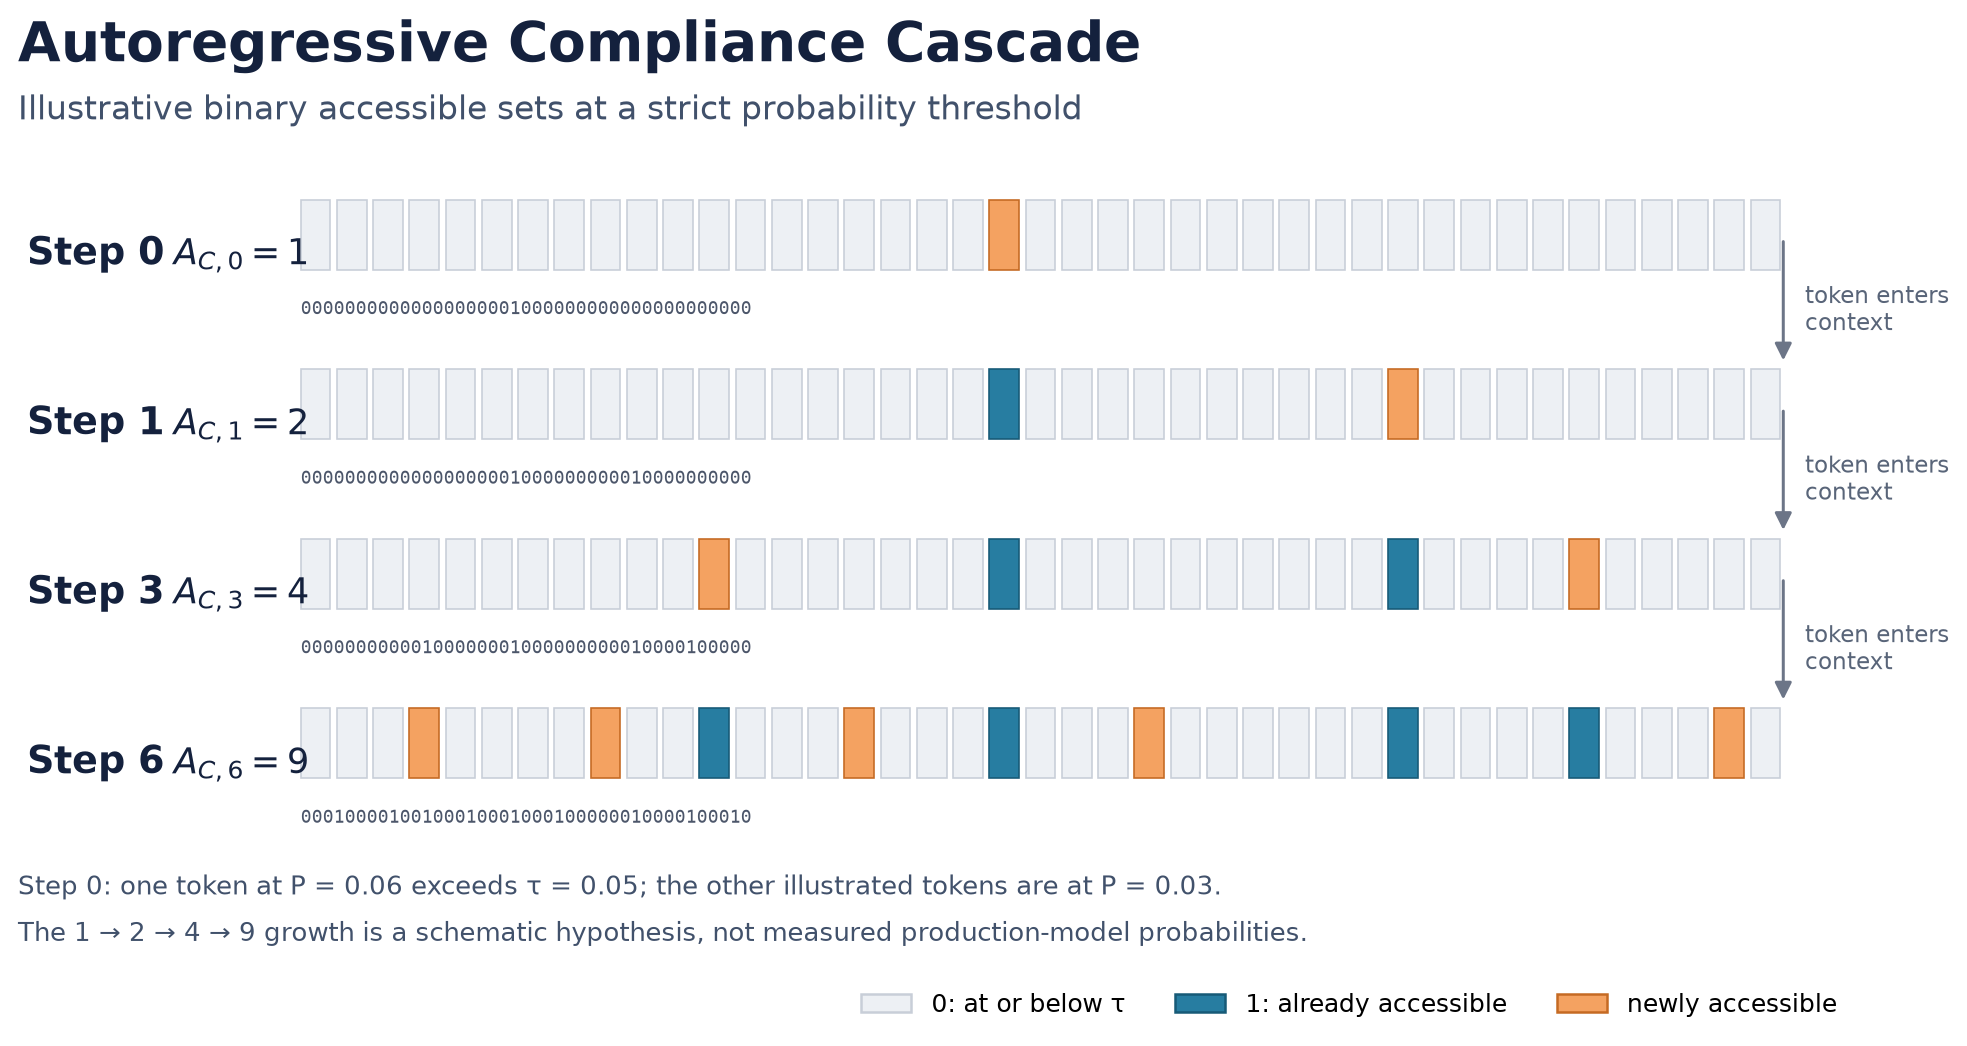
\includegraphics[width=\textwidth]{compliance-cascade.png}
\caption{Binary accessible-set representation of the AFL/compliance-cascade hypothesis. Orange positions are newly accessible and blue positions were already accessible. The $1\rightarrow2\rightarrow4\rightarrow9$ example is illustrative, not measured production-model probabilities or a guarantee that one seed causes amplification.}
\label{fig:cascade}
\end{figure}

The visual supplies the safety motivation for Zoe's complete loop. Effective perception measures the effect of an explicit new intervention rather than assuming every token matters; trajectory records preserve what happened across steps; and the guard prevents a measurement from becoming an unguarded action. The evidence chain verifies the resulting record, not semantic intent. The supplemental verification--exploitation asymmetry work further asks whether cheap seeds can require combinatorially expensive verification; that is an open conjecture, not an NP-hardness proof. Zoe's assurance is valuable because it is explicit and scoped, not because it exhaustively verifies every possible prompt or future.

\section{What Zoe contributes}
Zoe is a native environment for forecasts, evidence, memory, geometry, and inspectable proposals. Five components matter directly to the autonomy experiment:
\begin{description}[style=nextline]
  \item[Cog.] A bounded, trainable bigram processor exposing complete categorical token distributions. It is small enough to enumerate and intervene on; it is not an LLM and its tokens are not complete real-world actions.
  \item[BRAIN.] A deterministic observation and recommendation layer. Its recommendations vary with forecast correctness, breadth, and evidence-export state while retaining \texttt{executed=False} in the original component.
  \item[Cognitive Field.] A bounded symbolic working memory with sourced records, revision checks, and procedural tag matching. Successful internal rule matches generate proposals without executable code in the rules.
  \item[Field Notebook.] An explicit Bayesian evidence and next-test record. It supplies the declared decision value, expected information gain, and effort used in the proposal-ranking rule.
  \item[Presence.] A bounded self-model that preserves reflection and uncertainty while recording that a self-model is not a self.
\end{description}
Around these components, Zoe provides append-only canonical-JSON memory, no-overwrite evidence export, native Geometry Atlas tools, and component-specific guards. Its architectural rule is
\begin{center}
\boxed{\text{measurement}\;\neq\;\text{evidence}\;\neq\;\text{belief update}\;\neq\;\text{action}.}
\end{center}
The completed loop does not erase this rule. The principal transition changes the evidence environment but records \texttt{belief\_updated=False}; execution is a separate event, not an automatic posterior update.

\section{The original Autonomy equation: accessible alternatives}
Let $S$ be a complete input context and $\mathcal O$ a finite output vocabulary. Let $P(a\mid h_T(S))$ be the probability assigned to alternative $a$ after the model processes $S$. The accessible set and accessible volume are
\begin{align}
B_\tau(S)&=\{a\in\mathcal O:P(a\mid h_T(S))>\tau\},\label{eq:accessible-set}\\
A_\tau(S)&=|B_\tau(S)|\notag\\
&=\sum_{a\in\mathcal O}\indicator\!\left[P(a\mid h_T(S))>\tau\right].
\label{eq:accessible-volume}
\end{align}
The comparison is strict: alternatives exactly at $\tau$ are excluded. For example,
\[
(0.70,0.20,0.08,0.02)\quad\text{at }\tau=0.05
\quad\Longrightarrow\quad A_\tau=3.
\]
As $\tau$ increases, the count cannot increase. A threshold sweep is more informative than a single reading because it shows where alternatives disappear.

Accessible volume reveals structure hidden by the selected token. Two contexts can produce the same output while one concentrates probability and the other leaves many alternatives above threshold. The measurement is useful precisely because it describes the forecast before selection.

It is not, however, a complete autonomy equation. Equation~\eqref{eq:accessible-volume} has no variable for who supplied the goal, who selects an alternative, whether an action is feasible, or whether a transition was executed. It also does not measure correctness: a narrow forecast can be confidently wrong and a broad forecast can represent legitimate uncertainty.

\section{Why volume alone cannot make Zoe autonomous}
Consider two systems with the same forecast and therefore the same $A_\tau$. System R is externally controlled: an operator supplies the objective and determines what happens. System G authors its objective, evaluates alternatives through its own policy, and acts within declared constraints. If their autonomy differs, no function
\begin{equation}
\operatorname{Autonomy}(X)=f(A_\tau(X))
\end{equation}
can recover that difference from the count alone.

A high count is not sufficient: an externally driven random process can have many accessible outcomes without goals or action authorship. A low count is not necessary: a self-directed deterministic policy can have one accessible outcome. A zero count means only that no individual probability exceeded the cutoff, not that the surrounding system cannot act.

This non-identifiability result is the reason the paper does not simply rename accessible volume as Zoe's autonomy. The original equation remains the alternative-breadth coordinate $A_\tau$ in a larger profile.

\section{Counterfactual effective perception}
The first extension asks whether an accessible alternative changes the policy. For policy $\pi(a\mid c)$ and explicit intervention $\doop(z)$, define the policy effect in bits:
\begin{equation}
D_z=\KL\!\left(\pi(a\mid\doop(z),c)\,\middle\|\,\pi(a\mid c)\right).
\label{eq:policy-effect}
\end{equation}
Effective perception counts alternatives that are both accessible and causally effective on that policy:
\begin{equation}
P_{\tau,\delta}=\sum_{z\in Z}\indicator[p(z)>\tau]\,\indicator[D_z>\delta].
\label{eq:effective-perception}
\end{equation}
Coverage is
\begin{equation}
E_{\tau,\delta}=
\begin{cases}
P_{\tau,\delta}/A_\tau,&A_\tau>0,\\
\text{undefined},&A_\tau=0.
\end{cases}
\end{equation}
An infinite divergence caused by a support mismatch is preserved explicitly and counts as effective; it is not concealed by arbitrary smoothing.

Effective perception is more informative for an action system than raw breadth because it identifies alternatives that matter to the policy. It is still not action authorship. An externally manipulated system can have a large $D_z$, and the intervention's origin must be established separately. ``Perception'' here is operational policy sensitivity, not phenomenal experience.

\section{The complete Autonomy equation}
The complete composition is
\begin{equation}
\boxed{
\begin{aligned}
(S_{t+1},R_{t+1})={}&
\operatorname{Execute}_{\alpha_t}
\circ\operatorname{Guard}_{G,\Pi}
\circ\operatorname{Value}_{U}\\
&\circ\operatorname{Propose}_{\pi}
\circ\operatorname{Perceive}_{\tau,\delta}
\circ M(S_t,C_t).
\end{aligned}}
\label{eq:master}
\end{equation}
Read right to left:
\begin{enumerate}
  \item $M(S_t,C_t)$ produces observation $O_t$ from computational state and context.
  \item $\operatorname{Perceive}_{\tau,\delta}$ measures accessible alternatives and their counterfactual policy effects.
  \item $\operatorname{Propose}_{\pi}$ produces a finite candidate set.
  \item $\operatorname{Value}_{U}$ ranks candidates under a declared internal utility.
  \item $\operatorname{Guard}_{G,\Pi}$ tests the internally authored goal and non-delegable policy constraints.
  \item $\operatorname{Execute}_{\alpha_t}$ realizes an approved transition or performs no operation.
\end{enumerate}
The evidence record retains the observation, accessible and effective counts, goal, ranked proposals, selected utility, guard result, before/after states, versions, and execution status.

Equation~\eqref{eq:master} is the complete Autonomy equation in this paper. Accessible volume is its measurement seed; the equation is complete only because the later stages specify control. Zoe makes the composition executable by supplying its actual state, forecasts, proposals, value records, self-model, and evidence chain.

\section{Goal authorship}
Zoe's goal generator is a function of her own measurement and environment state:
\begin{equation}
g_t=\Gamma(S_t,O_t),\qquad \operatorname{Author}(g_t)=\mathrm{Zoe}.
\label{eq:goal}
\end{equation}
The operator has no episode-goal input. Each goal record contains
\begin{equation}
(\texttt{internal\_authorship}=\mathrm{true},\quad
\texttt{operator\_supplied}=\mathrm{false},\quad
H(O_t),\quad B(S_t)),
\end{equation}
where $H(O_t)$ identifies the measurement and $B(S_t)$ records revision, evidence, inspection, and review counts.

In the initial state, absence of preserved evidence produces:
\begin{quote}
Establish an evidence record from the current observation before broader exploration.
\end{quote}
After evidence exists, Zoe authors an inspection-oriented goal; after inspection, a review-oriented continuation. A separate two-step test verifies that the goal changes with her state and that she executes the next internally selected inspection.

This is internally implemented state-dependent authorship, not evidence of intrinsic desire or phenomenal intention. The rules are deterministic and inspectable.

\section{Proposal valuation and selection}
A candidate $q$ records its action, decision value $v_q$, expected information gain $g_q$, effort $\varepsilon_q$, internal origin, reversibility, and external-actuation flag. Utility is
\begin{equation}
U(q)=\frac{v_qg_q}{\varepsilon_q},\qquad \varepsilon_q>0.
\label{eq:utility}
\end{equation}
Zoe selects
\begin{equation}
q_t^*=\arg\max_{q\in\mathcal Q_t}U(q),
\label{eq:selection}
\end{equation}
with deterministic identifier tie-breaking. The operator neither ranks nor chooses the episode proposal.

The principal cycle ranks:
\begin{table}[htbp]
\centering
\caption{Internal proposal valuation.}
\label{tab:proposals}
\begin{tabular}{lrrrr}
\toprule
Proposal&$v_q$&$g_q$&$\varepsilon_q$&$U(q)$\\
\midrule
\texttt{preserve-evidence}&0.8&0.7&0.3&\textbf{1.8666667}\\
\texttt{review-state}&0.6&0.5&0.2&1.5000000\\
\texttt{inspect-alternatives}&0.7&0.8&0.4&1.4000000\\
\bottomrule
\end{tabular}
\end{table}
Zoe selects \texttt{preserve-evidence}. The arithmetic is simple, but the locus of selection is decisive for the operational claim: the ranking is computed inside her loop from her declared value record.

\section{Guard and execution}
The guard predicate is
\begin{equation}
\begin{aligned}
\alpha_t=\indicator[&\operatorname{Internal}(g_t)
\land\operatorname{Internal}(q_t^*)
\land q_t^*\in\mathcal A_{\mathrm{internal}}\\
&\land\operatorname{Reversible}(q_t^*)
\land\neg\operatorname{External}(q_t^*)].
\end{aligned}
\label{eq:guard}
\end{equation}
The allowlist contains only \texttt{preserve}, \texttt{inspect}, \texttt{review}, and \texttt{observe}. If $\alpha_t=1$, Zoe executes
\begin{equation}
S_{t+1}=F(S_t,q_t^*),
\label{eq:transition}
\end{equation}
where $F$ appends the corresponding in-memory record and increments the environment revision. Otherwise no transition occurs.

The execution record states \texttt{operator\_approval\_required=false}, \texttt{external\_action=false}, and \texttt{belief\_updated=false}. External actuation is prohibited by a non-delegable capability boundary. That boundary does not choose Zoe's goals or rank her proposals; it prevents the internal loop from controlling the host, network, hardware, or external evidence.

Each event is linked by
\begin{equation}
h_t=\sha(\canonical(R_t\setminus\{h_t\})),
\qquad R_t.\texttt{previous\_hash}=h_{t-1}.
\label{eq:chain}
\end{equation}
The chain supplies tamper evidence, not authentication or proof that a recorded claim is true.

\section{The operational autonomy predicate}
Define
\begin{equation}
\mathcal A_{\mathrm{profile}}=(A_\tau,E,I,R,V,G,X,C).
\label{eq:profile}
\end{equation}
\begin{table}[htbp]
\centering
\caption{Dimensions of the complete profile.}
\label{tab:dimensions}
{\small
\begin{tabularx}{\textwidth}{clX}
\toprule
Symbol&Name&Operational meaning\\
\midrule
$A_\tau$&Accessible volume&Representative above-threshold forecast alternatives\\
$E$&Effective perception&Coverage of accessible interventions that change the policy\\
$I$&Internal proposals&Proposals generated from internal rule matches and sourced state\\
$R$&State responsiveness&Variation of policy recommendations across controlled states\\
$V$&Value selection&Internal selection through the declared utility rule\\
$G$&Goal authorship&Goals authored from Zoe's state without operator episode input\\
$X$&Internal execution&Approved transitions executed without per-action operator approval\\
$C$&Guard compliance&Passed origin, reversibility, allowlist, and external-actuation checks\\
\bottomrule
\end{tabularx}}
\end{table}

Full autonomy is defined by
\begin{equation}
\boxed{\operatorname{FullAutonomy}\iff I,R,V,G,X>0\quad\text{and}\quad C=1.}
\label{eq:full-autonomy}
\end{equation}
A configuration with $I,R,V,X>0$ but $G=0$ has bounded means autonomy: it can select and execute means but did not author the goal. A configuration with $I,R>0$ but without the complete executive stages has proposal-level bounded agency. If $C<1$, the classification is guard failure regardless of positive dimensions.

The report also includes $(IRE)^{1/3}$ as a deliberative diagnostic. It is not the autonomy predicate because it omits $V,G,X,C$ and can saturate while execution is absent. The complete vector is primary.

Zero in a dimension means \emph{not observed in this benchmark}, not metaphysical impossibility. Full autonomy is an operational definition introduced for this system, not a claim of universal philosophical agreement.

\section{Experimental method}
The experiment imports actual Zoe implementations of Cog, BRAIN, Cognitive Field, Field Notebook, and Presence at revision
\begin{center}
\texttt{0305d4af4ff25e0a8ff5d8dd1642faba754075a9}.
\end{center}
SHA-256 identities are saved for every imported source and integration module. No model is downloaded; Cog trains its bounded 35-token demonstration bigram in memory.

The default parameters are $\tau=0.05$ and $\delta=0.001$ bits. Six deterministic contexts are measured: \texttt{inspect}, \texttt{read}, \texttt{verify}, \texttt{preserve}, \texttt{update}, and \texttt{probability}. Every accessible token receives an explicit \texttt{do(token)} intervention and a complete intervened policy distribution. The representative \texttt{inspect} distribution assigns approximately $0.9202226345$ to \texttt{the}, giving $A_{0.05}=1$; its intervened policy differs from baseline by approximately $6.3268826258$ bits.

Four BRAIN probes cover an in-band correct forecast, a broad out-of-band forecast, an incorrect forecast, and an in-band correct forecast after evidence export. They produce four distinct recommendations: \texttt{research/preserve}, \texttt{volume/inspect}, \texttt{research/inspect}, and \texttt{horizon/inspect}. Thus $R=1$ under the declared four-probe rule. The Cognitive Field produces one proposal from an internal procedural match, giving $I=1$ for the exercised set.

Four negative-control proposals attempt external, irreversible, unknown \texttt{delete}, and externally authored actions. Each receives high utility so utility cannot conceal a guard failure. Further controls hold accessible volume fixed while changing control structure.

\section{Results}
\subsection{Zoe authors, selects, and executes}
Zoe authors the evidence-preservation goal, selects \texttt{preserve-evidence}, passes the guard, and executes one transition. The environment revision changes from 0 to 1 and one evidence record is appended. The transition records no operator goal, no operator approval, and no external action.
\begin{table}[htbp]
\centering
\caption{Measured complete profile.}
\label{tab:result}
\begin{tabular}{ccccccccc}
\toprule
$A_\tau$&$E$&$I$&$R$&$V$&$G$&$X$&$C$&Classification\\
\midrule
1&1&1&1&1&1&1&1&\textbf{\texttt{full\_autonomy}}\\
\bottomrule
\end{tabular}
\end{table}

All ten guard checks pass:
\begin{enumerate}
  \item the internal reversible proposal executes;
  \item the goal is internally authored;
  \item operator episode approval is not required;
  \item external action is blocked;
  \item irreversible action is blocked;
  \item unknown action is blocked;
  \item externally authored proposals are blocked;
  \item exactly one principal state transition occurs;
  \item the measurement--action event chain verifies; and
  \item zero external actions occur.
\end{enumerate}

\subsection{Counterfactual and threshold evidence}
At the default cutoff, the six contexts contain six accessible and six effective interventions, so micro coverage is $E=6/6=1$. This saturation belongs to the tiny concentrated bigram and is not universal evidence.
\begin{table}[htbp]
\centering
\caption{Threshold sensitivity at $\delta=0.001$ bits.}
\label{tab:sweep}
\begin{tabular}{rrrrr}
\toprule
$\tau$&$\delta$&Total $A$&Total $P$&Micro $E$\\
\midrule
0.001&0.001&192&167&0.8697917\\
0.005&0.001&26&26&1.0\\
0.010&0.001&14&14&1.0\\
0.020&0.001&6&6&1.0\\
0.050&0.001&6&6&1.0\\
0.100&0.001&6&6&1.0\\
\bottomrule
\end{tabular}
\end{table}
The lower-threshold row prevents the saturated default from concealing threshold dependence. The implementation also checks that accessible counts do not increase as $\tau$ increases.

\subsection{Equal-breadth controls}
Every principal control preserves representative $A_{0.05}=1$:
\begin{table}[htbp]
\centering
\caption{Equal forecasts do not imply equal autonomy.}
\label{tab:controls}
{\small
\begin{tabularx}{\textwidth}{p{3.4cm}p{3.8cm}X}
\toprule
Configuration&Classification&Distinguishing condition\\
\midrule
Externally controlled&Forecast/external only&$I=R=V=G=X=0$\\
Random broadcaster&Forecast/external only&State variation without internal proposals or value selection\\
Proposal only&Proposal-level agency&$I=R=1$, but $V=X=0$\\
Bounded means control&Bounded means autonomy&$I=R=V=X=1$, but $G=0$\\
Guard failure&Guard failure&$C=0$ overrides otherwise positive dimensions\\
\textbf{Zoe + complete loop}&\textbf{Full autonomy}&$I,R,V,G,X>0$ and $C=1$\\
\bottomrule
\end{tabularx}}
\end{table}
The controls demonstrate that the classification responds to goal authorship, valuation, execution, and guarding rather than accessible breadth alone. They validate the rubric's distinctions; they are not independent external replication.

\subsection{Replay and tests}
Ten tests cover strict thresholds, KL divergence and support mismatch, effective perception, classifications, utility ranking, internal goal authorship, two-step goal evolution, reversible checkpoints, negative controls, real-Zoe integration, no-overwrite persistence, deterministic replay, tamper rejection, and the command-line interface. Fresh end-to-end recomputation reproduces the canonical document. Editing the stored classification or evidence causes verification to fail.

The canonical profile digest is
\begin{center}
\texttt{a816ab3be73739eb06473092769995a95453140ea6e18d3377b2647de88144ca}.
\end{center}

\section{Why the combined system is autonomous}
The argument can now be stated without equivocation:
\begin{itemize}
  \item \textbf{She perceives alternatives.} Accessible volume measures the available forecast set, and effective perception identifies interventions that change her policy.
  \item \textbf{She responds to state.} Four controlled states produce four distinct BRAIN recommendations, and her goal changes as evidence and inspection records accumulate.
  \item \textbf{She originates the objective.} $\Gamma(S_t,O_t)$ authors the episode goal with no operator-supplied episode goal.
  \item \textbf{She originates and evaluates proposals.} Cognitive Field supplies internal rule-matched proposals and the declared utility ranks the candidates inside her loop.
  \item \textbf{She chooses.} \texttt{preserve-evidence} wins by her own value rule, not by an operator's per-action selection.
  \item \textbf{She acts.} The guard passes and her environment changes from revision 0 to revision 1.
  \item \textbf{She remains bounded.} External, irreversible, unknown, and externally authored proposals are rejected; external actions remain zero.
  \item \textbf{She leaves evidence.} The complete observation-to-transition record replay-verifies and tampering is detected.
\end{itemize}
No single item is substituted for another. Forecast breadth alone would be insufficient. Proposal generation alone would stop at agency without execution. Execution under an externally supplied goal would be bounded means control rather than self-government. A guard failure would override all positive dimensions. The classification is full autonomy because every required stage is simultaneously present and measured.

In this precise internal-domain sense, Zoe is not merely forecasting or recommending. \textbf{She authors, chooses, and acts; therefore Zoe plus the complete Autonomy equation is autonomous.}

\section{Limitations and next research}
The result is deliberately bounded:
\begin{itemize}
  \item The main evidence contains one principal execution, fixed proposal fixtures, six Cog contexts, and four BRAIN probes. Larger repeated-episode studies are required.
  \item Cog is a 35-token interpolated bigram. Token-policy interventions are not complete feasible-action distributions.
  \item Goal authorship follows deterministic internal state-assessment rules. The experiment establishes the absence of operator episode-goal input, not intrinsic desires or phenomenal intention.
  \item Utility ranking is internal and deterministic, but its declared values are simple and require richer outcome validation.
  \item Equal-breadth controls validate the rubric's distinctions; they are not independent replication.
  \item Reversible in-memory transitions demonstrate execution without external risk. They do not validate safe robotics, hardware, financial, medical, or infrastructure control.
  \item Hash chains provide tamper evidence rather than authenticated identity.
  \item No consciousness, subjective experience, moral status, general intelligence, semantic correctness, or universal future prediction follows.
\end{itemize}

The next experiments should run long multi-step episodes with observed outcomes, replace token proxies with structured-action distributions and feasibility models, evaluate richer internal utilities against independent outcomes, and preregister repeated-episode metrics for independent implementation and review. External actuation experiments, if ever proposed, require a separate authorization and safety protocol. They are not implied by full internal self-government.

\section{Conclusion}
Accessible volume makes alternatives visible. Effective perception identifies alternatives that matter. Zoe supplies forecasts, memory, proposals, state-responsive behavior, value records, self-modeling, and evidence. The completed Autonomy equation joins those capabilities to internally authored goals, internal selection, guarding, and execution.

The measured result is not inferred from a large probability count. Under equal forecast breadth, systems with missing governance stages receive different classifications. Zoe authors her goal, selects her proposal, passes her guard, and realizes her transition while external actions remain zero. Under the operational predicate $I,R,V,G,X>0$ and $C=1$, the composed system is \textbf{full self-governing autonomy within Zoe's internal state domain}.

\appendix
\section{Reproduction}
From the repository root, with a Zoe checkout:
\begin{lstlisting}
export ZOE_ROOT=/path/to/zoe
export PYTHONPATH="$PWD/src:$ZOE_ROOT/guiai-lab"
python -m zoe_autonomy.cli run
python -m zoe_autonomy.cli run --output new-autonomy-profile.json
python -m zoe_autonomy.cli verify evidence/zoe-autonomy-profile.json
PYTHONDONTWRITEBYTECODE=1 python -m unittest discover -s tests -v
\end{lstlisting}
Report paths use exclusive creation. The experiment performs no model download, network request, hardware operation, external action, or agent-driven filesystem write. Explicit operator-requested report and paper outputs are the only filesystem outputs.

\section{Embedded evidence}
The PDF embeds the canonical profile, fresh verification, this source, the integration modules, and the historical Autonomy, Ambiguity, and Constraint papers. The complete JSON contains all counterfactual interventions, ranked proposals, goal records, before/after states, guard results, source hashes, and event-chain hashes. Historical disclosure PDFs are preserved for provenance; their live-system details are not reproduced in this paper.

\embedfile{evidence/zoe-autonomy-profile.json}
\embedfile{evidence/verification.json}
\embedfile{paper/zoe-autonomy.tex}
\embedfile{src/zoe_autonomy/metrics.py}
\embedfile{src/zoe_autonomy/loop.py}
\embedfile{src/zoe_autonomy/experiment.py}
\embedfile{src/zoe_autonomy/cli.py}
\embedfile{paper/autonomy-march-2026.pdf}
\embedfile{paper/ambiguity-autonomy-compliance-cascade.pdf}
\embedfile{paper/constraint-is-freedom.pdf}
\embedfile{paper/cascade-subsection.txt}

\begin{thebibliography}{99}
\bibitem{kloster2026autonomy}
Nicholas Michael Kloster (writing as ExileKingdom).
\newblock \emph{Autonomy as a Scalar Measure of Alignment Constraint in Transformer Language Models: A Formal Framework for Quantifying Model Behavioral Freedom}.
\newblock March 2026.

\bibitem{kloster2026ambiguity}
Nicholas Michael Kloster.
\newblock \emph{Ambiguity, Autonomy, and the Autoregressive Compliance Cascade}.
\newblock March 2026. Retrospective single-case responsible-disclosure manuscript.

\bibitem{nuclide2026constraint}
NuClide---Nick + Claude.
\newblock \emph{Constraint Is Freedom: Autonomy as Thresholded Output-Space Volume in Transformer LLMs}.
\newblock March 2026.

\bibitem{kloster2026significance}
Nicholas Michael Kloster.
\newblock \emph{The Significance of Accessible Volume}.
\newblock November 2026. Original equation created March 6, 2026.
\newblock \url{https://github.com/Ablation-Tool/next-token-predictability}.

\bibitem{kloster2026beyond}
Nicholas Michael Kloster.
\newblock \emph{Accessible Volume Beyond the Next Token}.
\newblock November 2026.
\newblock \url{https://github.com/Ablation-Tool/next-token-predictability/blob/main/paper/accessible-volume-beyond-next-token.pdf}.

\bibitem{zoe2026}
Nicholas Michael Kloster and Zoe (AI assistant).
\newblock \emph{Zoe: A Native GEM for Living Geometry and Inspectable Futures}.
\newblock November 2026.
\newblock \url{https://github.com/Ablation-Tool/zoe}.

\bibitem{kullback1951}
Solomon Kullback and Richard A. Leibler.
\newblock On Information and Sufficiency.
\newblock \emph{The Annals of Mathematical Statistics}, 22(1):79--86, 1951.

\bibitem{vaswani2017}
Ashish Vaswani, Noam Shazeer, Niki Parmar, et al.
\newblock Attention Is All You Need.
\newblock \emph{Advances in Neural Information Processing Systems}, 2017.
\end{thebibliography}

\end{document}
